% Especificaciones del tamaño de letra, tamaño de hoja, márgenes, librerias, etc.
\documentclass[12pt, letterpaper]{article}
\usepackage[english]{babel}
\usepackage{fancyhdr}
\usepackage[utf8]{inputenc}
\usepackage[T1]{fontenc}
\usepackage{amsmath}
\usepackage{graphicx}
\usepackage{subcaption}
\usepackage[hidelinks]{hyperref}
\usepackage{url}
\usepackage{amssymb}
\usepackage{float}
\usepackage[margin=1in]{geometry}
\usepackage{listings}
\usepackage{verbatim}
\usepackage[most]{tcolorbox} % Produces color boxes.
\renewcommand{\baselinestretch}{1.5}

\lstset{numbers=left}
% Enlace Bibliografía
\usepackage{csquotes}
\usepackage[notes,backend=biber]{biblatex-chicago}
\addbibresource{referencias.bib}

% Titulo, autores, fecha.
\title{Práctica \#4: Diseño de un Perfil NACA}
\author{Carlos A. Vásquez Castañeda \and 1155057 \and Grupo 395}
\date{Marzo 21, 2020}
\pagestyle{fancy}
\fancyhf{}
\rhead{Mecánica de Sustentación}
\lhead{Práctica \#4}
\rfoot{\thepage}

\definecolor{lightgreen}{RGB}{255, 128, 159}
% Inicio del documento
\begin{document}
\maketitle

\section*{Introducción}
La dinámica de fluidos computacional (CDF por sus siglas en inglés) se enfoca en el análisis de sistemas que involucran fluidos. transferencia de calor y fenómenos relacionados como lo son reacciones químicas, y esto es posible a través de la simulación por computadoras. Esta técnica tiene mucho poder y un gran rango de aplicaciones, desde lo industrial hasta áreas de investigación. Algunos ejemplos son:

\begin{itemize}
	\item aerodinámica en una aeronave y automóviles: sustentación y arrastre.
	\item hidrodinámica de barcos.
	\item plantas de energía: combustión en motores de combustión interna y turbinas de gas.
	\item ingeniería eléctrica y electrónica: enfriamiento de equipo eléctrico, incluyendo microcircuitos.
	\item ingeniería marina.
	\item ingeniería renovable.
	\item hidrología y oceanografía.
\end{itemize}

Desde la década de los 1960 hasta el presente, la industria aeroespacial ha integrado técnicas de la dinámica de fluidos computacional en el diseño, manufactura de aeronaves y motores, etc. 

Una de las metas principales de los desarrollos en estas técnicas es ayudar a realizar herramientas con una capacidad comparable a aquellas ingenierías que trabajan con software CAD para, por ejemplo,  el análisis de esfuerzos en una viga. Las ténicas de la dinámica de fluidos computacional se han atrasado considerablemente en comparación a las CAD debido a la gran complejidad de los problemas analizados en esta área. Con los últimos avances tecnológicos y la optimización del código que se encuentra en nuestros ordenadores, es posible crear estos entornos que hace unas décadas era imposible de llevar acabo. Todo esto tiene sus ventajas y desventajas. Las simulaciones y análsis se volvieron más fácil de realizar, sin embargo tienen un costo muy grande debido al desarrollo de software capaz de realizar estos análisis de manera confiable.


\subsection*{Funcionamiento}

Los códigos y programas utilizados para la resolución de estos problemas están estructurados entorno a algoritmos numéricos que sean capaces de llegar a una solución a estos problemas de fluidos. Se cuenta con una etapa de pre-procesamiento, solucionador y post-procesamiento.

En la etapa de \textbf{pre-procesamiento} se define la geometría de la región de interés. En esta etapa también se lleva acabo la generación de una cuadrícula o malla, esto para subdividir el dominio definido por la geometría dada, los cuales contienen \textit{volúmenes de control} donde se llevarán acabo la resolución de estas ecuaciones de manera numérica.

En esta etapa también se definen las propiedades del fluido, fenómenos físicos y químicos que necesitan modelarse y especificaciones de condiciones de frontera (debido a que los modelos utilizados son ecuaciones diferenciales complejas y necesitan estas condiciones para obtener un resultado físico significativo.)

La solución a estos problemas (velocidad, presión, temperatura, etc.) está definida en nodos dentro de cada volumen de control. La precisión y exactitud de la solución generada por el programa dependerá del número de celdas (o volúmenes de control) con los que se disponga. Las mallas más óptimas son no uniformes: más finas en las área con una gran variación de punto a punto, y menos detalladas en las regiones donde hay poco cambio. El 50\% de el tiempo que se dispone en la industria está destinado solamente a la definición de la geometría y la malla a generar, es por esto que se buscan nuevas maneras de optimizar este proceso de pre-procesamiento.

La etapa de \textbf{solución} depende de gran medida de el distribuidor del código a utilizar, sin embargo la mayoría utilizan el método de volumen finito, similar al análisis de elemento finito. En esta etapa se integran las ecuaciones que gobieranan el comportamiento del fluido y su flujo a lo largo de las celdas establecidas en la geometría, la discretización (conversión de las ecuaciones integales resultantes a sistemas de ecuaciones algebráicas) y la solución de las ecuaciones algebráicas utilizando métodos iterativos (donde los ordenadores logran destacar más).

Por último, la etapa de \textbf{post-procesamiento} simplemente se encarga de ilustrar de manera gráfica los resultados obtenidos en la etapa de solución. Las paqueterías que se encargan de la resolución de estos problemas están equipadas actualmente con muchas herramientas que permiten la visualización de datos de manera muy versátil. Esto incluye campos vectoriales, campos escalares, gráficas de contorno, gráficas de superficies bidimensionales y tridimensionales, rastreo de partículas, manipulación de la vistas tridimensionales, entre más opciones.

\section*{Procedimiento de la Práctica}

Antes de comenzar a realizar el modelo como tal del perfil alar, es necesario contar con estos perfiles estandarizados. La página de la NACA cuenta con distintos perfiles normalizados, en archivos $.dat$ para el uso y análisis público de éstos. En esta ocasión analizaremos un perfil NACA 4412. Los datos sobre estos puntos son descargados y posteriormente los utilizaremos.

Estos datos ya son bastante útiles como tal, sin embargo es incómodo trabajar con ellos de la manera en la que está dispuesta la estructura de datos, además de que se nos pide analizar este perfil con un largo de cuerda de 50 mm. Por suerte estos datos se encuentran normalizados, lo cual quiere decir que podemos reajustarlos de manera sencilla. Para esto hay muchos métodos posibles y el que expondré en esta ocasión es uno basado en un procesador de texto y hojas de cálculo. 

Dada la naturaleza del archivo $.dat$, es posible editarlos de manera sencilla. Utilizando \textit{Vim} podemos recurrir a distintas maneras de realizar la edición.

\begin{figure}[H]
	\centering
	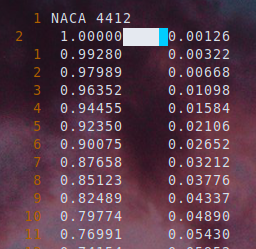
\includegraphics[width=0.3\textwidth]{01.png}
	\caption{Estructura de datos con las coordenadas X y Y de los puntos del perfil alar.}
\end{figure}

Como podemos observar en la figura anterior, el archivo $.dat$ tiene una estructura consistente, donde sólo el primer renglón es distinto, y los demás renglones comienzan con un espacio, el dato de la coordenada X, seguido de cinco espacios y el dato de la coordenada Y. A través de \textit{Vim} es posible reemplazar estos espacios con comas (,) con el siguiente comando.
\begin{tcolorbox}[
	enhanced,
	attach boxed title to top left={xshift=6mm,yshift=-3mm},
	colback=white,
	colframe=lightgreen!10,
	colbacktitle=lightgreen!10,
	title=Comando de Vim,
	fonttitle=\bfseries\color{black},
	boxed title style={size=small,colframe=white!20,sharp corners},
	sharp corners,
] % General configuration for the color box, wrapping the code.

\begin{lstlisting}[language=bash]
:%s/     /,/g
\end{lstlisting}
\end{tcolorbox}

Con esto reemplazamos sólo la sucesión de cinco espacios que se encuentran en todas las líneas con una coma, los espacios singulares siguen quedando al inicio de todas las líneas. Dada esta situación, también es posible eliminar los espacios singulares con un comando similar, que los reemplace con un caracter nulo. Una vez hecho esto, nuestra estructura de datos quedará de la siguiente manera.

\begin{figure}[H]
	\centering
	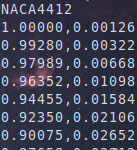
\includegraphics[width=0.2\textwidth]{02.png}
	\caption{Estructura de datos acomodada.}
\end{figure}

Quizá resulte extraño haberle dado ese formato a los datos, sin embargo resulta muy útil si transformamos esa estructura de datos de un archivo $.dat$ a un archivo $.csv$, donde las columnas son separadas por comas. Este tipo de archivo es posible abrirlo en una hoja de cálculo, por lo que programas como Excel y LibreOffice nos permitirán editarlo con más opciones aún.

Abriendo este archivo en LibreOffice, realizaremos otra columna que contenga solamente el número 1, esto porque el formato de \textit{SpaceClaim} está hecho de esta manera para realizar el posicionamiento y trazado entre los puntos indicados (esa primer coordenada se toma como el eje Z). Después, cada dato lo multiplicaremos por 50, dado que nuestra longitud de cuerda es de 50, pero la que se encuentra en los datos es de 1. Hecho esto tendremos algo similar a esto:

\begin{figure}[H]
	\centering
	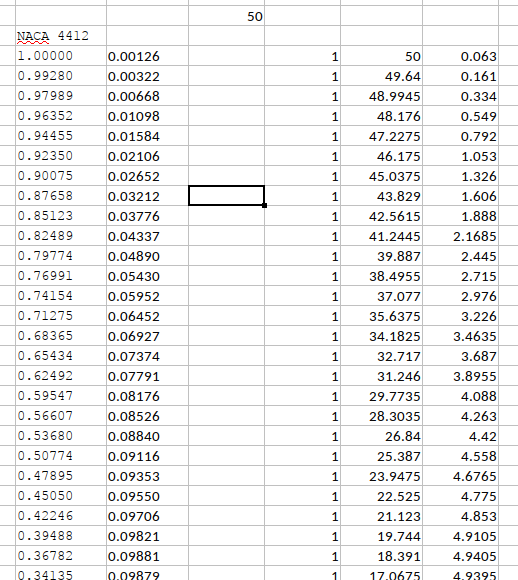
\includegraphics[width=0.7\textwidth]{03.png}
	\caption{Nuevos datos creados en la hoja de cálculo.}
\end{figure}

Las tres últimas columnas son de interés ya que estos datos son los que leerá ANSYS. Lo único que queda hacer es guardar estas columnas en un archivo $.txt$ de la siguiente manera:

\begin{figure}[H]
	\centering
	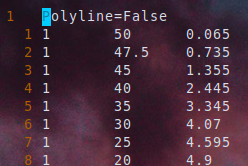
\includegraphics[width=0.4\textwidth]{04.png}
	\caption{Creación del archivo "data.txt"}
\end{figure}

Estos datos están separados por una indentadura ([TAB]) y la primer línea tiene una configuración para ANSYS. Con este archivo ahora procedemos a cargarlo al programa mediante la opción de ANSYS para abrir documentos.

\begin{figure}[H]
	\centering
	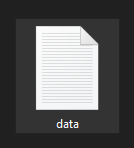
\includegraphics[width=0.2\textwidth]{1.png}
	\caption{Carga del archivo de los puntos.}
\end{figure}

Automáticamente se cargará y se trazará el perfil alar con los puntos posicionados.

\begin{figure}[H]
	\centering
	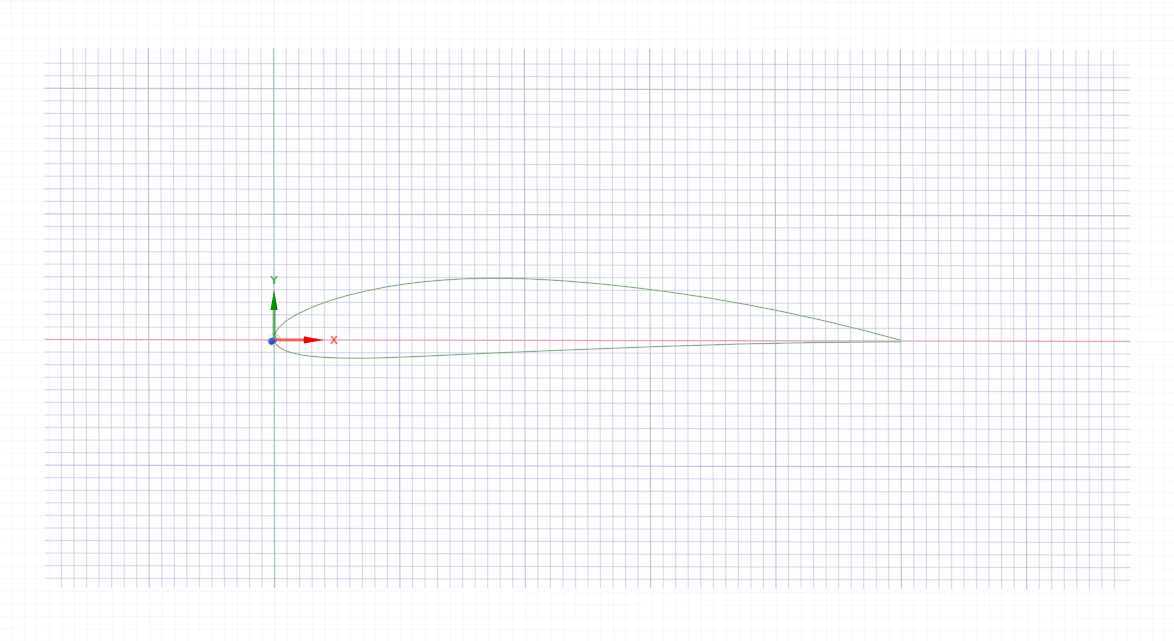
\includegraphics[width=0.7\textwidth]{2.png}
	\caption{}
\end{figure}

Por más útil que esto sea, es importante revisar la topología de nuestra superficie ya que en ocasiones ANSYS podrá trazar las lineas uniendo los puntos, pero no siempre será capaz de inferir cómo cerrar las curvas que introduzcamos, por eso con la herramienta de línea es posible trazar una línea que una los dos últimos vértices de la curva.

\begin{figure}[H]
	\centering
	\begin{subfigure}[b]{0.49\linewidth}
		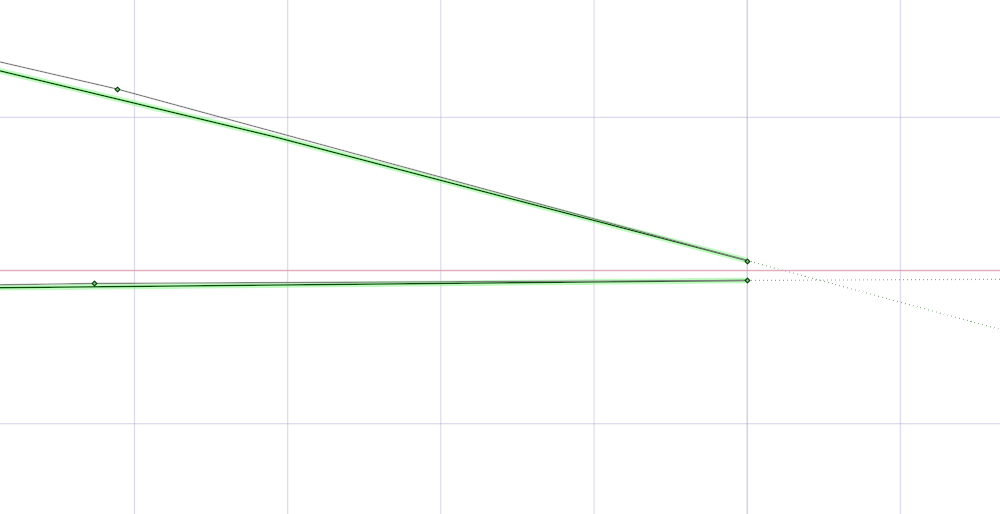
\includegraphics[width=\linewidth]{3.png}
		\caption{Curva abierta}
	\end{subfigure}
	\begin{subfigure}[b]{0.49\linewidth}
		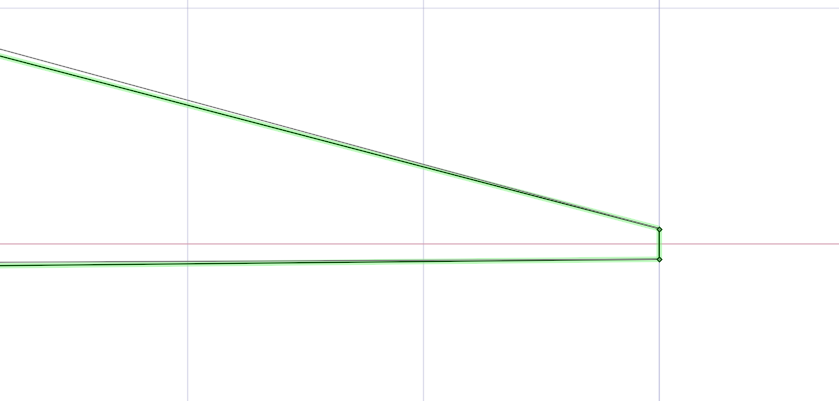
\includegraphics[width=\linewidth]{4.png}
		\caption{Curva cerrada.}
	\end{subfigure}
	\caption{Artefactos al momento de importar un conjunto de datos.}
\end{figure}

Una vez trazada la curva, se procede a realizar el trazo de un rectángulo. Este rectángulo funcionará como un "túnel de viento", y es importante ya que posteriormente sobre esta superficie se realizará un mallado para lograr implementar un análsis numérico y simulaciones de fluidos. Mientras tanto, se traza este rectángulo con las dimensiones indicadas.

\begin{figure}[H]
	\centering
	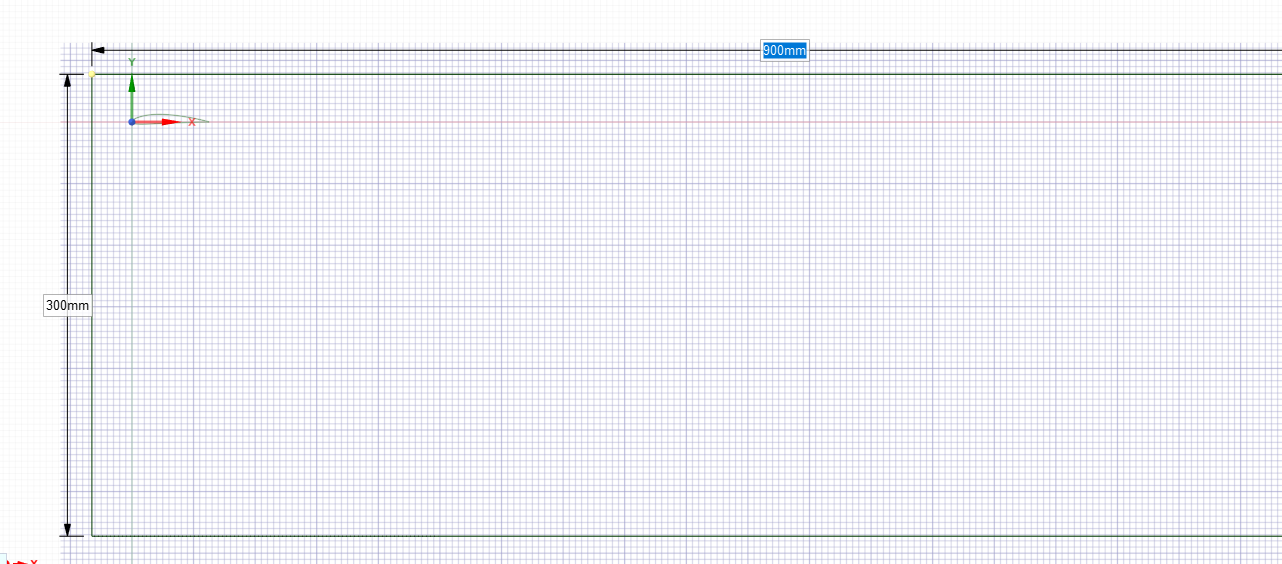
\includegraphics[width=\textwidth]{5.png}
	\caption{Rectángulo con dimensiones de 300 mm x 900 mm.}
\end{figure}

Una vez hecho este rectángulo, debemos de posicionar el perfil alar de la manera en la que se indicó, para esto debemos de utilizar la herramienta "Mover", y podremos posicionar nuestro perfil alar en el centro del rectángulo gracias a los centroides de las figuras.

\begin{figure}[H]
	\centering
	\begin{subfigure}[b]{0.49\linewidth}
		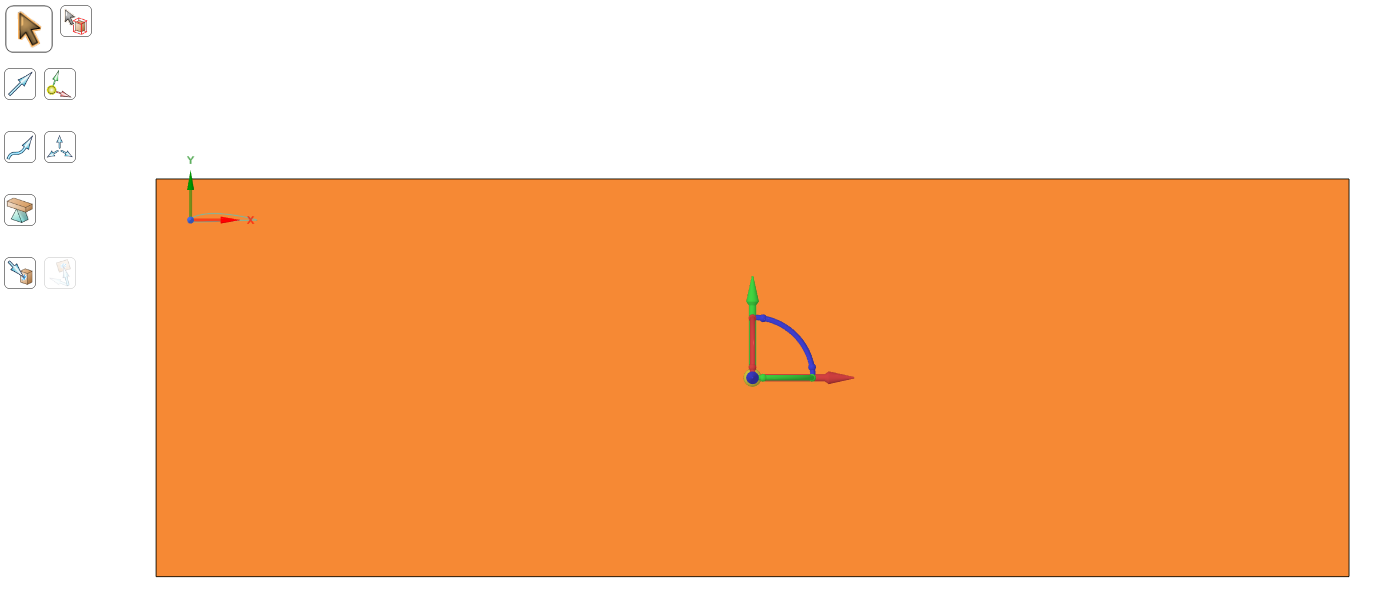
\includegraphics[width=\linewidth]{7.png}
		\caption{Antes de la transformación.}
	\end{subfigure}
	\begin{subfigure}[b]{0.49\linewidth}
		
\includegraphics[width=\linewidth]{9.png}
		\caption{Después de la transformación.}
	\end{subfigure}
	\caption{Alineamiento de ambos cuerpos geométricos.}
\end{figure}

Sin embargo, el perfil alar no se debe de encontrar en el centro ya que nuestras especificaciones no lo dan como tal, sino que se debe encontrar a 200 mm de la pared izquierda del rectángulo. Ya que en este punto nuestro perfil alar se encuentra en la coordenada (450, 150), lo que podemos hacer es mover el perfil 250 mm a la izquierda para posicionarlo en la coordenada (200, 150), y así tener la geometría que se necesita.

\begin{figure}[H]
	\centering
	\begin{subfigure}[b]{0.49\linewidth}
		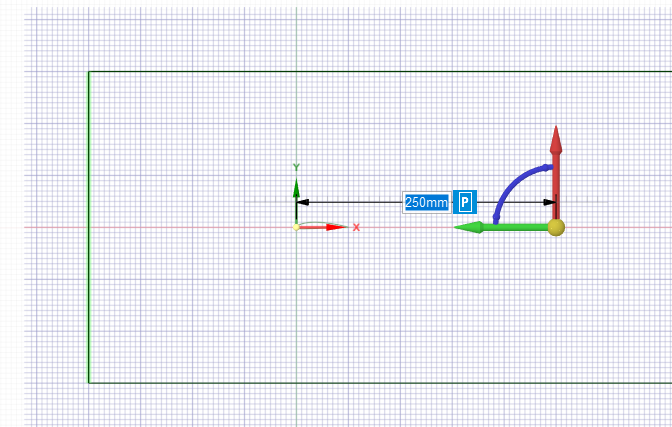
\includegraphics[width=\linewidth]{10.png}
		\caption{Movimiento de traslación}
	\end{subfigure}
	\begin{subfigure}[b]{0.49\linewidth}
		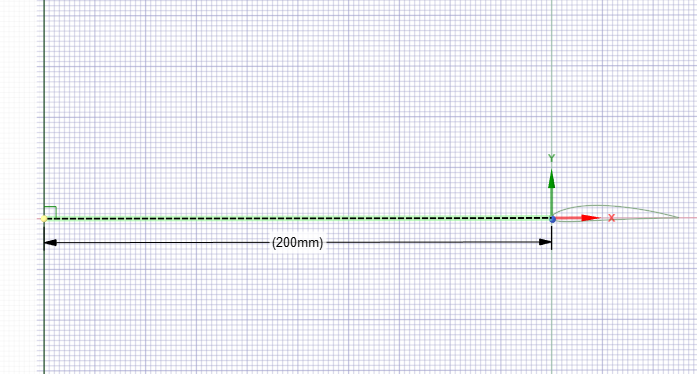
\includegraphics[width=\linewidth]{11.png}
		\caption{Medición de la pared al perfil alar.}
	\end{subfigure}
	\caption{Reposicionamiento del perfil.}
\end{figure}

Terminado esto, la curva se debe de proyectar en la superficie para hacer la diferenciación de estas dos. Esto se realiza mediante la opción de "Proyectar" en la sección "Intersecar" de ANSYS, lo cual hace un hueco en el rectángulo con la forma del perfil alar y sus dimensiones., lo cual hace un hueco en el rectángulo con la forma del perfil alar y sus dimensiones., lo cual hace un hueco en el rectángulo con la forma del perfil alar y sus dimensiones.

Después se realizará un recorte del perfil alar, se dividirá la parte superior de la inferior debido a que en el análisis se tienen que diferenciar para lograr obtener resultados de las distintas partes de la curva del perfil alar. Para esto se posiciona una línea de construcción a lo largo del eje longitudinal del perfil alar y se secciona en dos, como se muestra a continuación.

\begin{figure}[H]
	\centering
	\begin{subfigure}[b]{0.49\linewidth}
		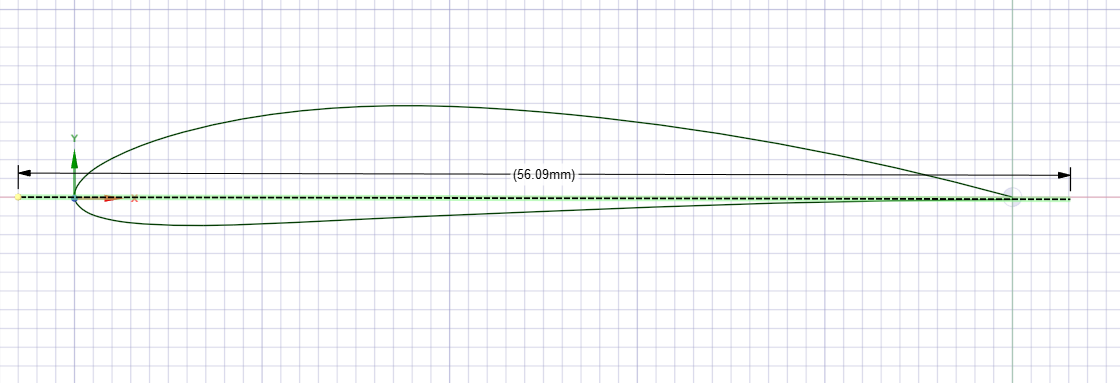
\includegraphics[width=\linewidth]{16.png}
		\caption{Curva antes de seccionar.}
	\end{subfigure}
	\begin{subfigure}[b]{0.49\linewidth}
		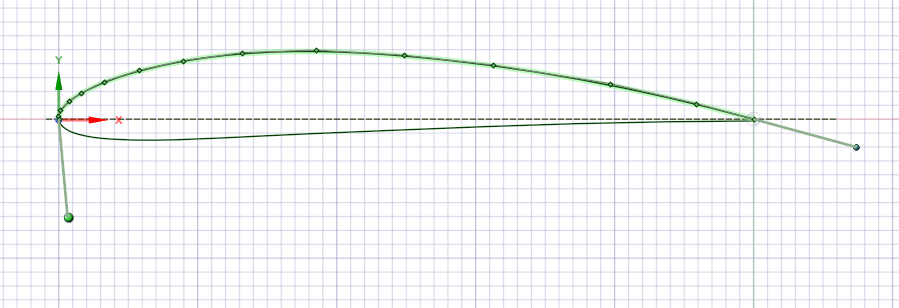
\includegraphics[width=\linewidth]{18.png}
		\caption{Curva después del seccionado.}
	\end{subfigure}
	\caption{División de la parte inferior y superior del perfil alar.}
\end{figure}


Saliendo a la vista 3D del modelo, podemos observar que nuestras superficies han sido diferenciadas y se ha hecho el modelo correctamente, lo que queda es seguir con la construcción del mallado y la simulación del fluido.

\begin{figure}[H]
	\centering
	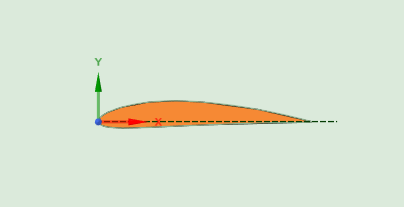
\includegraphics[width=\textwidth]{19.png}
	\caption{Superficie con el hueco del perfil alar.}
\end{figure}

\section*{Conclusión}

Hallar la geometría de los perfiles alares es en muchas ocasiones la tarea más difícil a realizar, sin embargo si se utilizan estandarizaciones como las de la NACA puede ser mucho más sencillo el modelado físico y virtual de estas geometrías. En esta ocasión se contó con el conjunto de datos que definían esta curva, pero en cualquier otro caso se debe de realizar un modelo en algún programa CAD para lograr importar una geometría como lo hicimos (o en su defecto, definir curvas paramétricas como lo hemos hecho en prácticas anteriores).

A pesar de haber hecho pasos muy sencillos en este reporte, es claro que es de los pasos más importantes. La geometría que hemos definido debe de quedar de manera correcta, no debe de haber discontinuidades y las medidas de distancia y dimensiones deben ser las correctas ya que estos resultados son nuestras especificaciones en el análisis del flujo de fluido, por lo que si tuviésemos condiciones iniciales un tanto más distintas, su solución sería completamente distinta. Esto debido a que la mecánica de fluidos tienen una naturaleza caótica, lo cual la vuelve virtualmente imposible de predecir en el futuro sin el conocimiento de las condiciones iniciales de cada partícula y un poder de procesamiento infinito.

Como exploramos en la introducción, estos pasos son los más importantes y a los que más se les dedica tiempo en la industria debido a su impacto en las soluciones que se obtendrán. Es por esto que una definición óptima de la geometría se tiene que realizar para obtener los resultados más cercanos a la realidad.

%%%%%  Bib
\renewcommand\refname{References}
\printbibliography
\end{document}
